\documentclass[12pt]{article}%
\usepackage{amsmath}
\usepackage{amssymb}
\usepackage{graphicx}


\begin{document}

\newcommand\scalemath[2]{\scalebox{#1}{\mbox{\ensuremath{\displaystyle #2}}}}
\title{Machine Learning \protect\\ Assignment 2 \protect\\ CLO3 Exercise 19} 
\author{Ida Bagus Dwi Satria Kusuma \protect\\ 1301140297}
\date{\today}
\maketitle

\begin{enumerate}
	\item In this exercise we will implement Probabilistic Neural Network (PNN) to classify data.
	\begin{enumerate}
		\item \textbf{(5 points)} Load the selected data set. Visualize all data points using scatter plot. Use different color or symbol for each class. Use attribute 1 as x -axis, attribute 2 as y -axis.

		\par \textbf{Jawab:} Visualisasi data menggunakan \textit{scatter plot}, di mana simbol 'o' merah adalah data dengan kelas '1', dan simbol 'segitiga' biru adalah data dengan kelas '2', dan '+' hijau adalah data dengan kelas '3'.
		\par 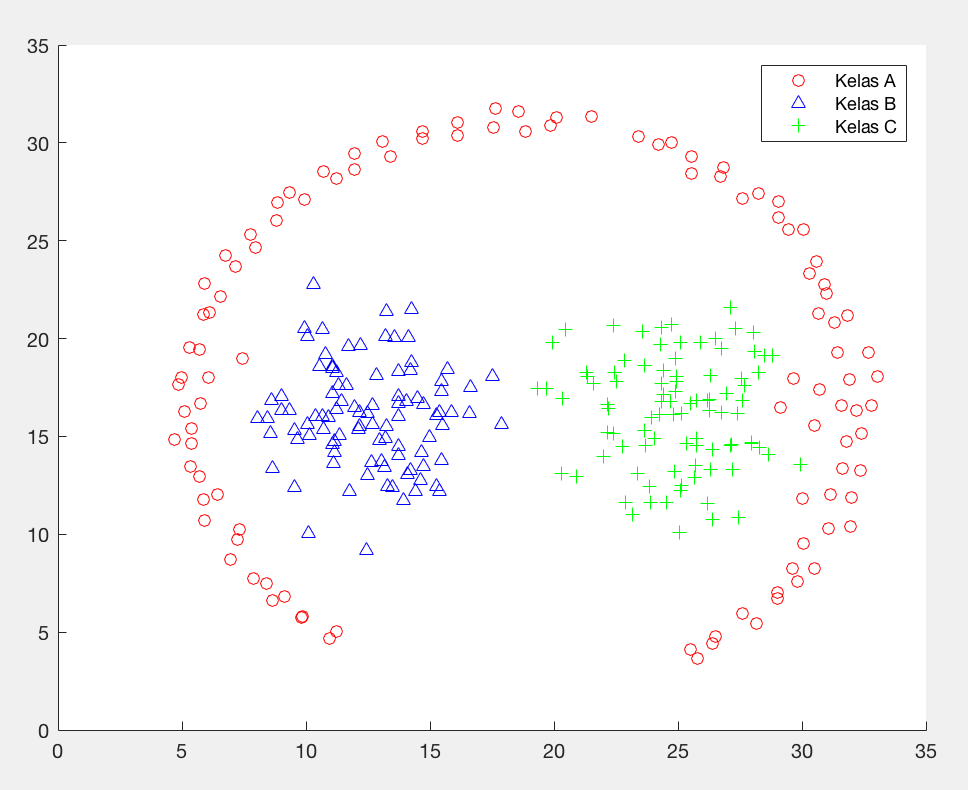
\includegraphics[width=10cm]{ass2clo3no19_1} 

		\item (10 points) Select randomly three data for test set (x′, y′), while remaining data as training set (x, y).

		\par Dengan menggunakan fungsi \textit{datasample} pada MATLAB, kita akan mendapatkan data untuk \textit{test set} secara acak.
		\par 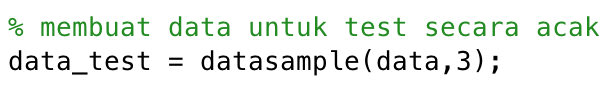
\includegraphics[width=10cm]{ass2clo3no19_2} 

		\item (15 points) Create a function that implements PNN. Inputs for the function are training set (x, y) and the attributes x′ of test set. The function outputs the predicted class yˆ for test set.

		\par Untuk mengimplementasikan PNN, kita menggunakan fungsi gaussian

		\[y = f(x_1,x_2) = \sum_{i=1}^{n} e^{\frac{-\left ( \left ( x_1-x_{1i} \right )^2+ \left ( x_2 - x_{2i} \right )^2\right ) }{2\delta^2}}\]

		\par Lalu, desain arsitektur PNN-nya 

		\par 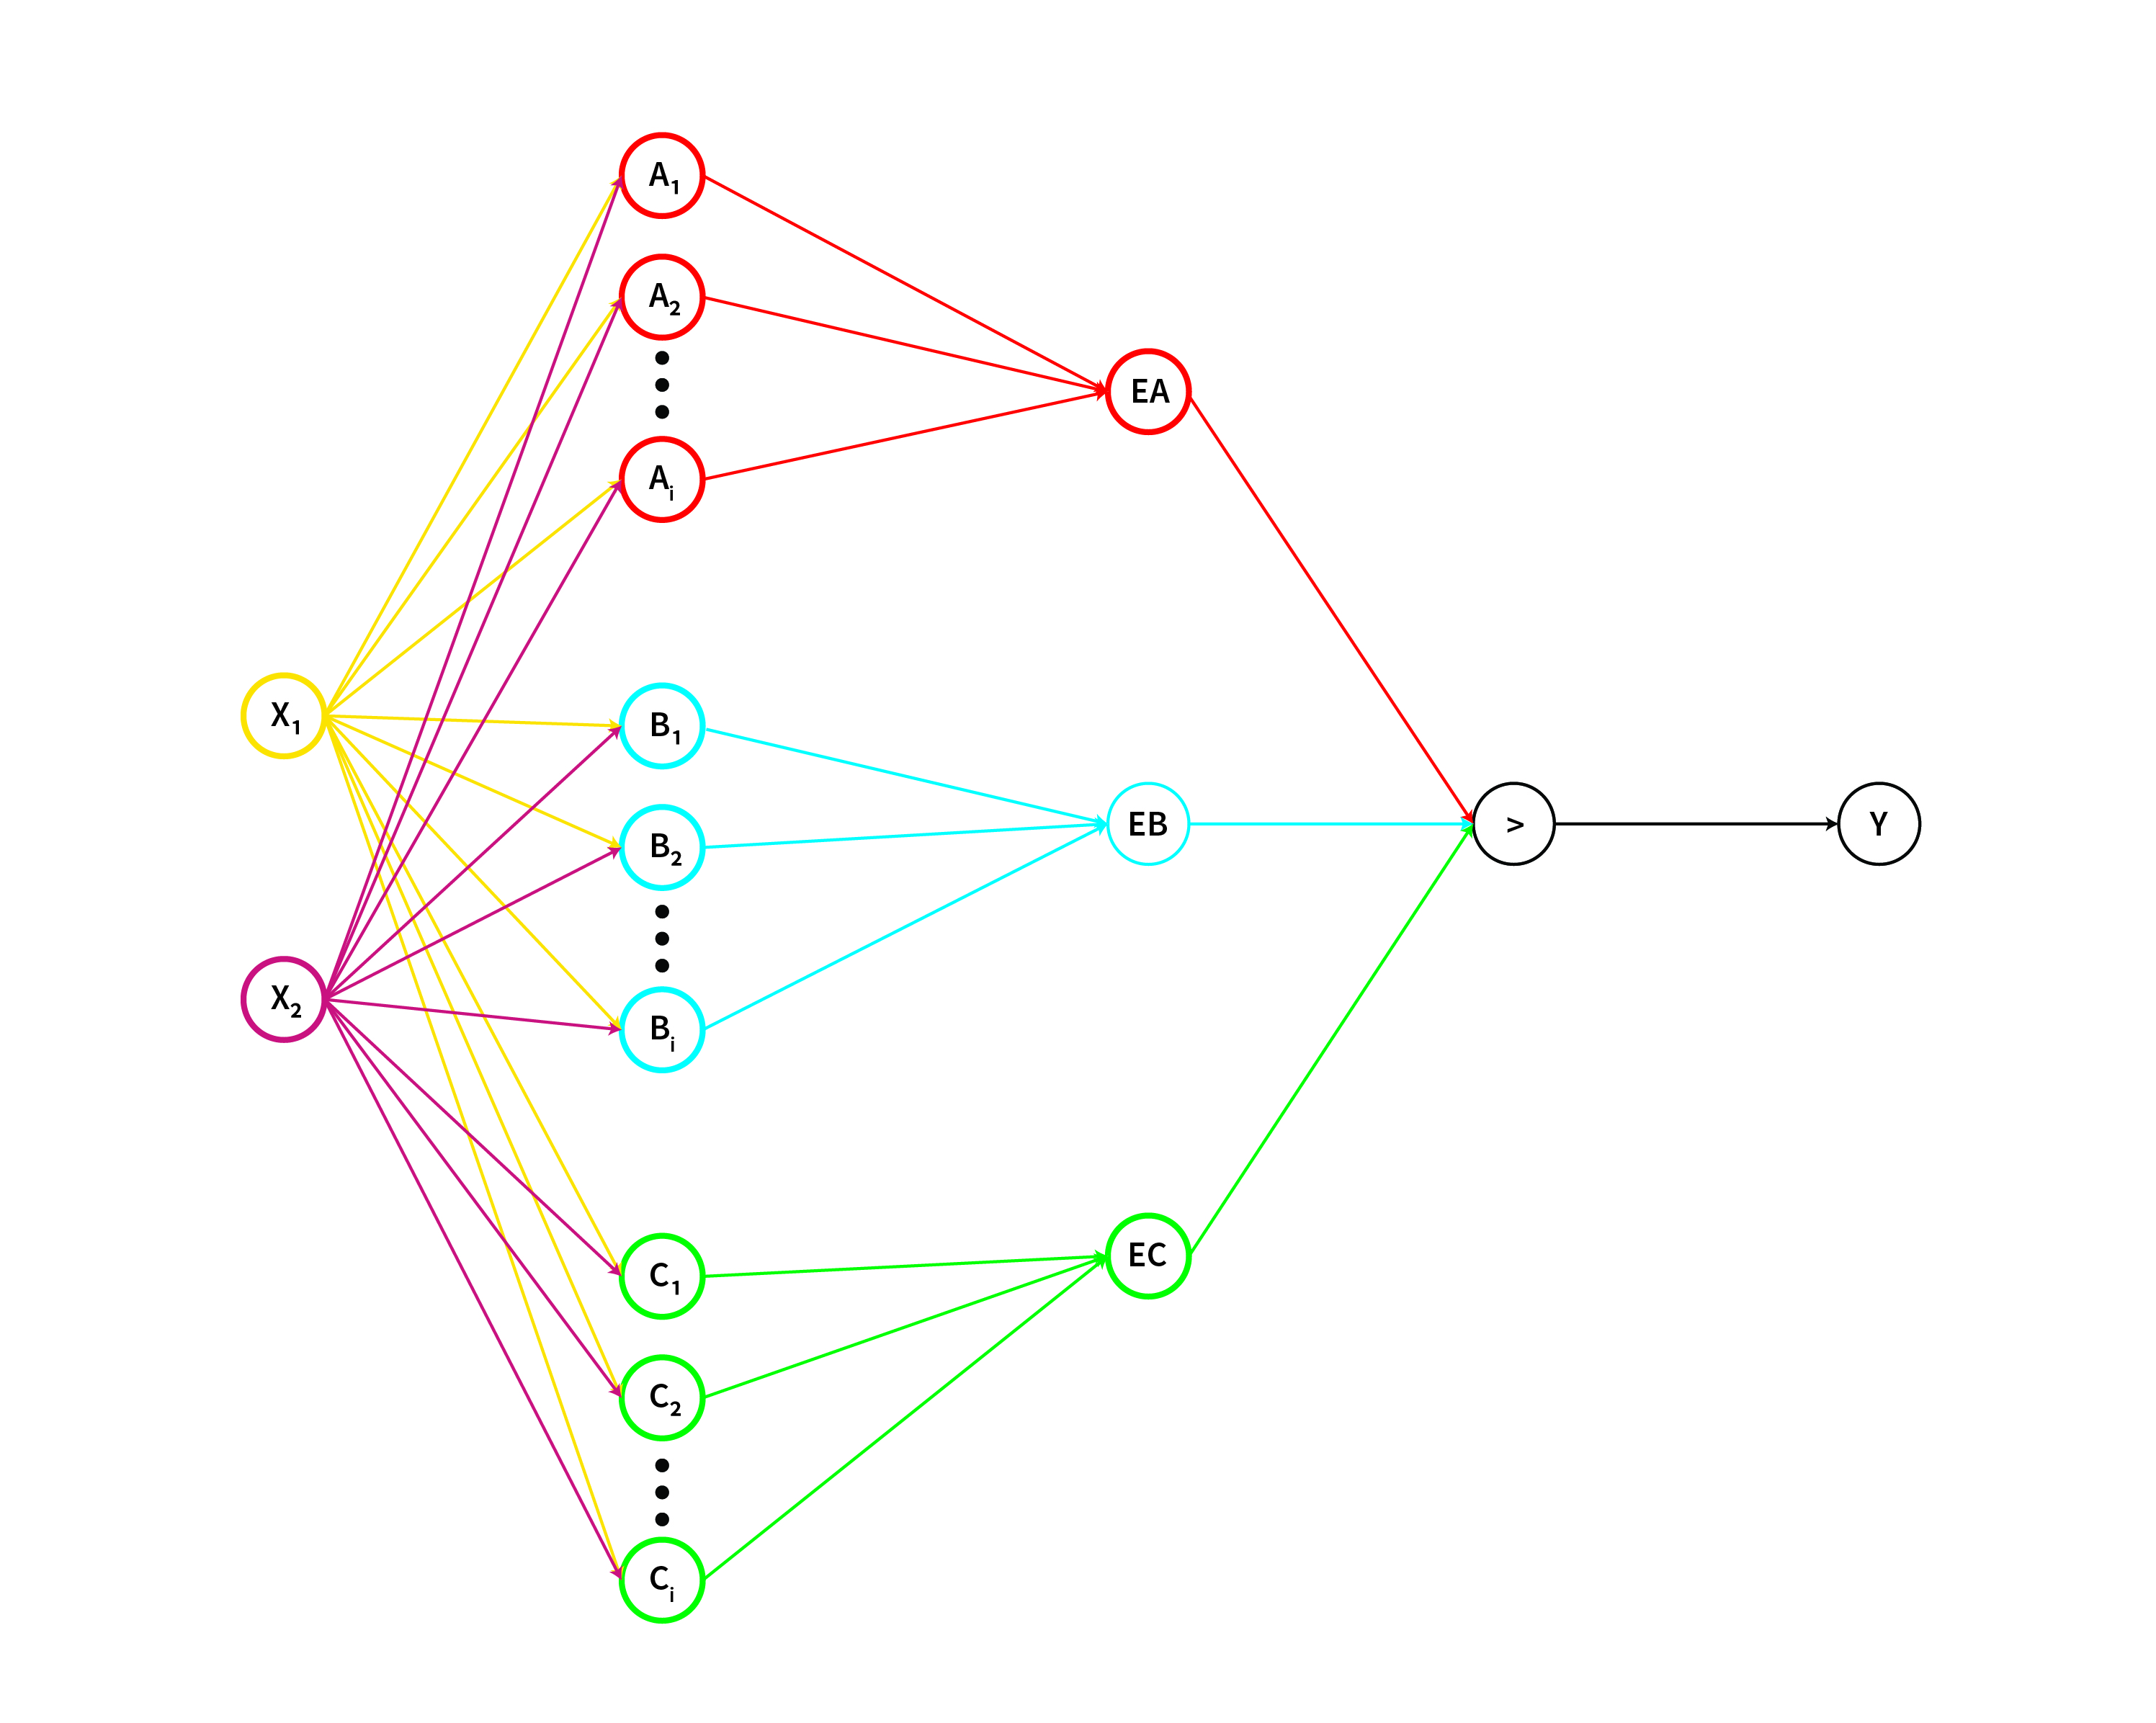
\includegraphics[width=10cm]{ass2clo3no19_3} 

		\par Code fungsi implementasi dari PNN :

		\par 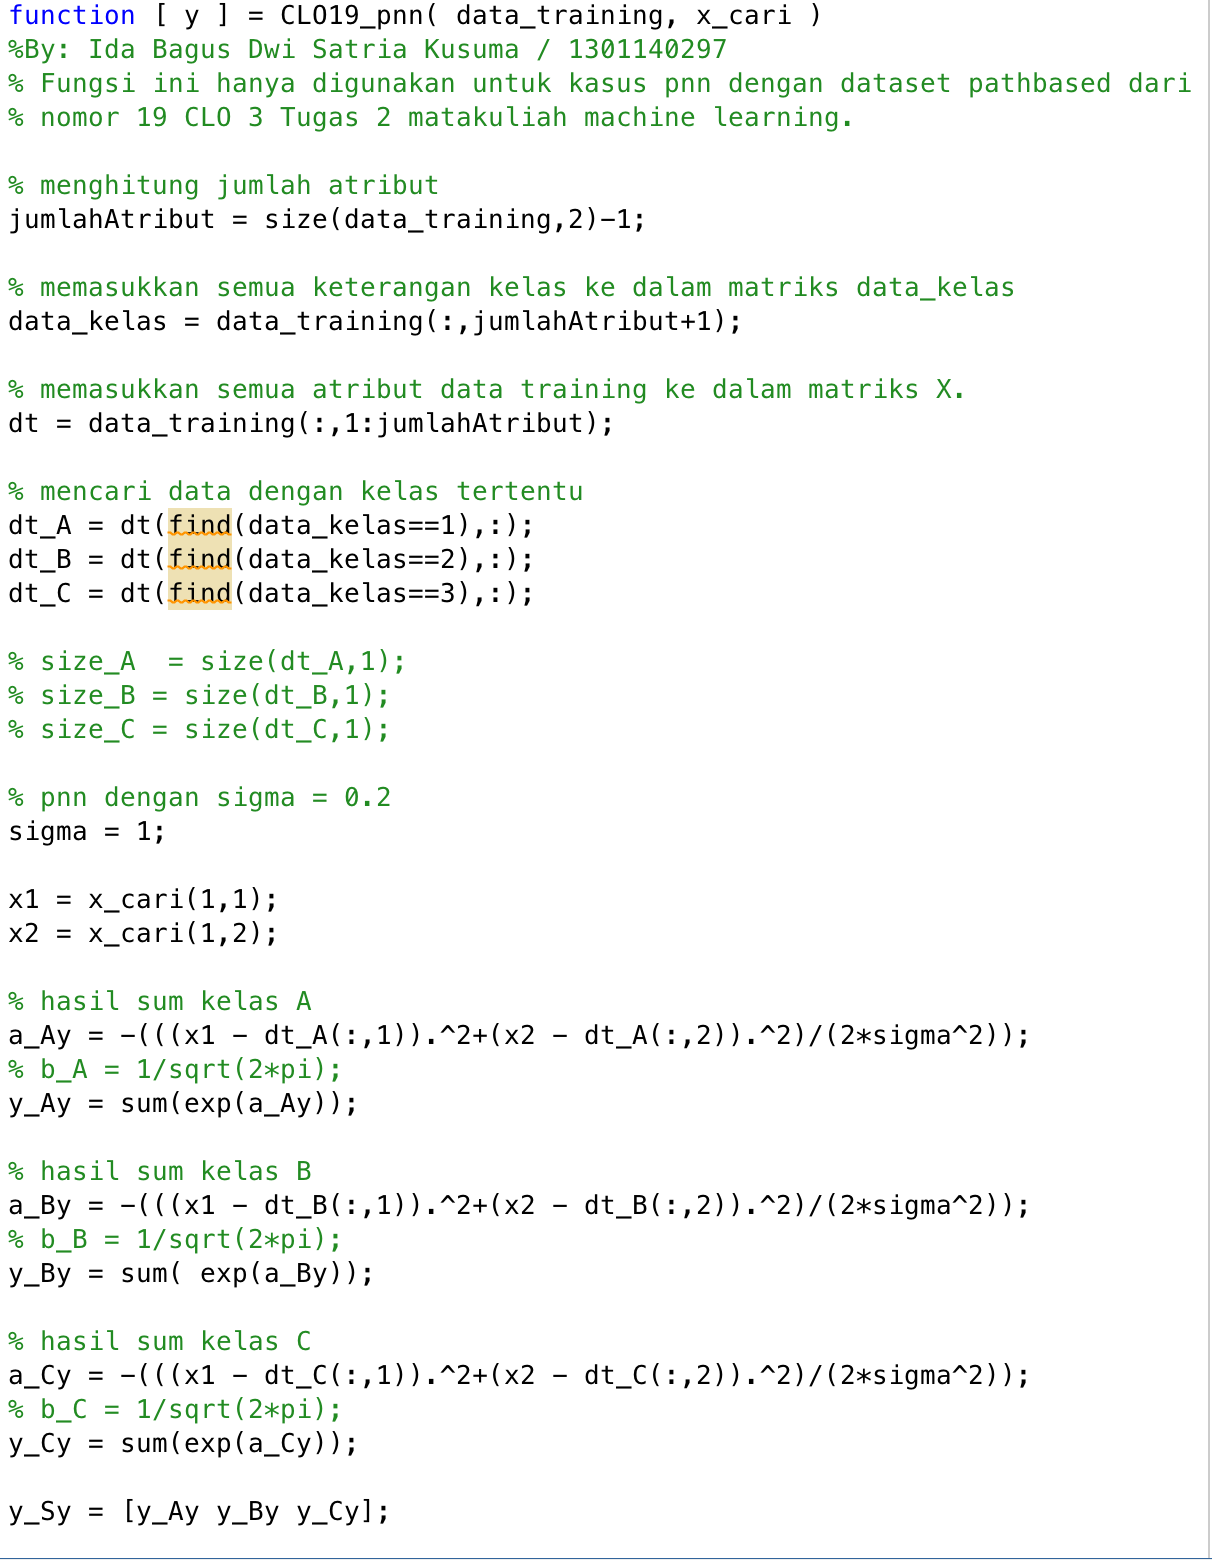
\includegraphics[width=10cm]{ass2clo3no19_4} 
		\par 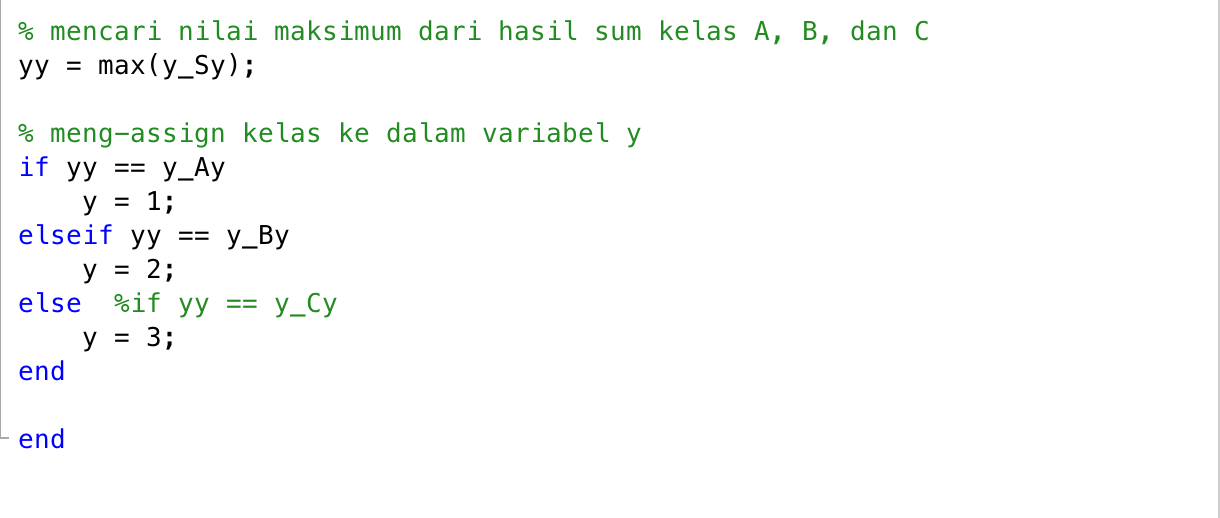
\includegraphics[width=10cm]{ass2clo3no19_5} 

		\item (5 points) Plot the decision boundary resulted from PNN classifier on the figure that has been created on 19(a). (Hints: First, generate data points using range of minimum and maximum value of each attribute, then classify each generated data points using the PNN classifier. Use attribute 1 and attribute 2 as x -axis and y -axis, respectively, of decision boundary location, while the predicted class label for giving coloring). One of online articles that you could learn on how to plot decision boundary using Octave/Matlab is here or go to the next url: http://www.peteryu.ca/tutorials/matlab/visualize\_decision\_boundaries. As alternative, you could use and modify a code program ’decbound2D’ that I sent to you. For python, Java, C++ and so on, you could search it on internet.

		\par Dengan memodifikasi fungsi decbound2D menjadi 

		\par 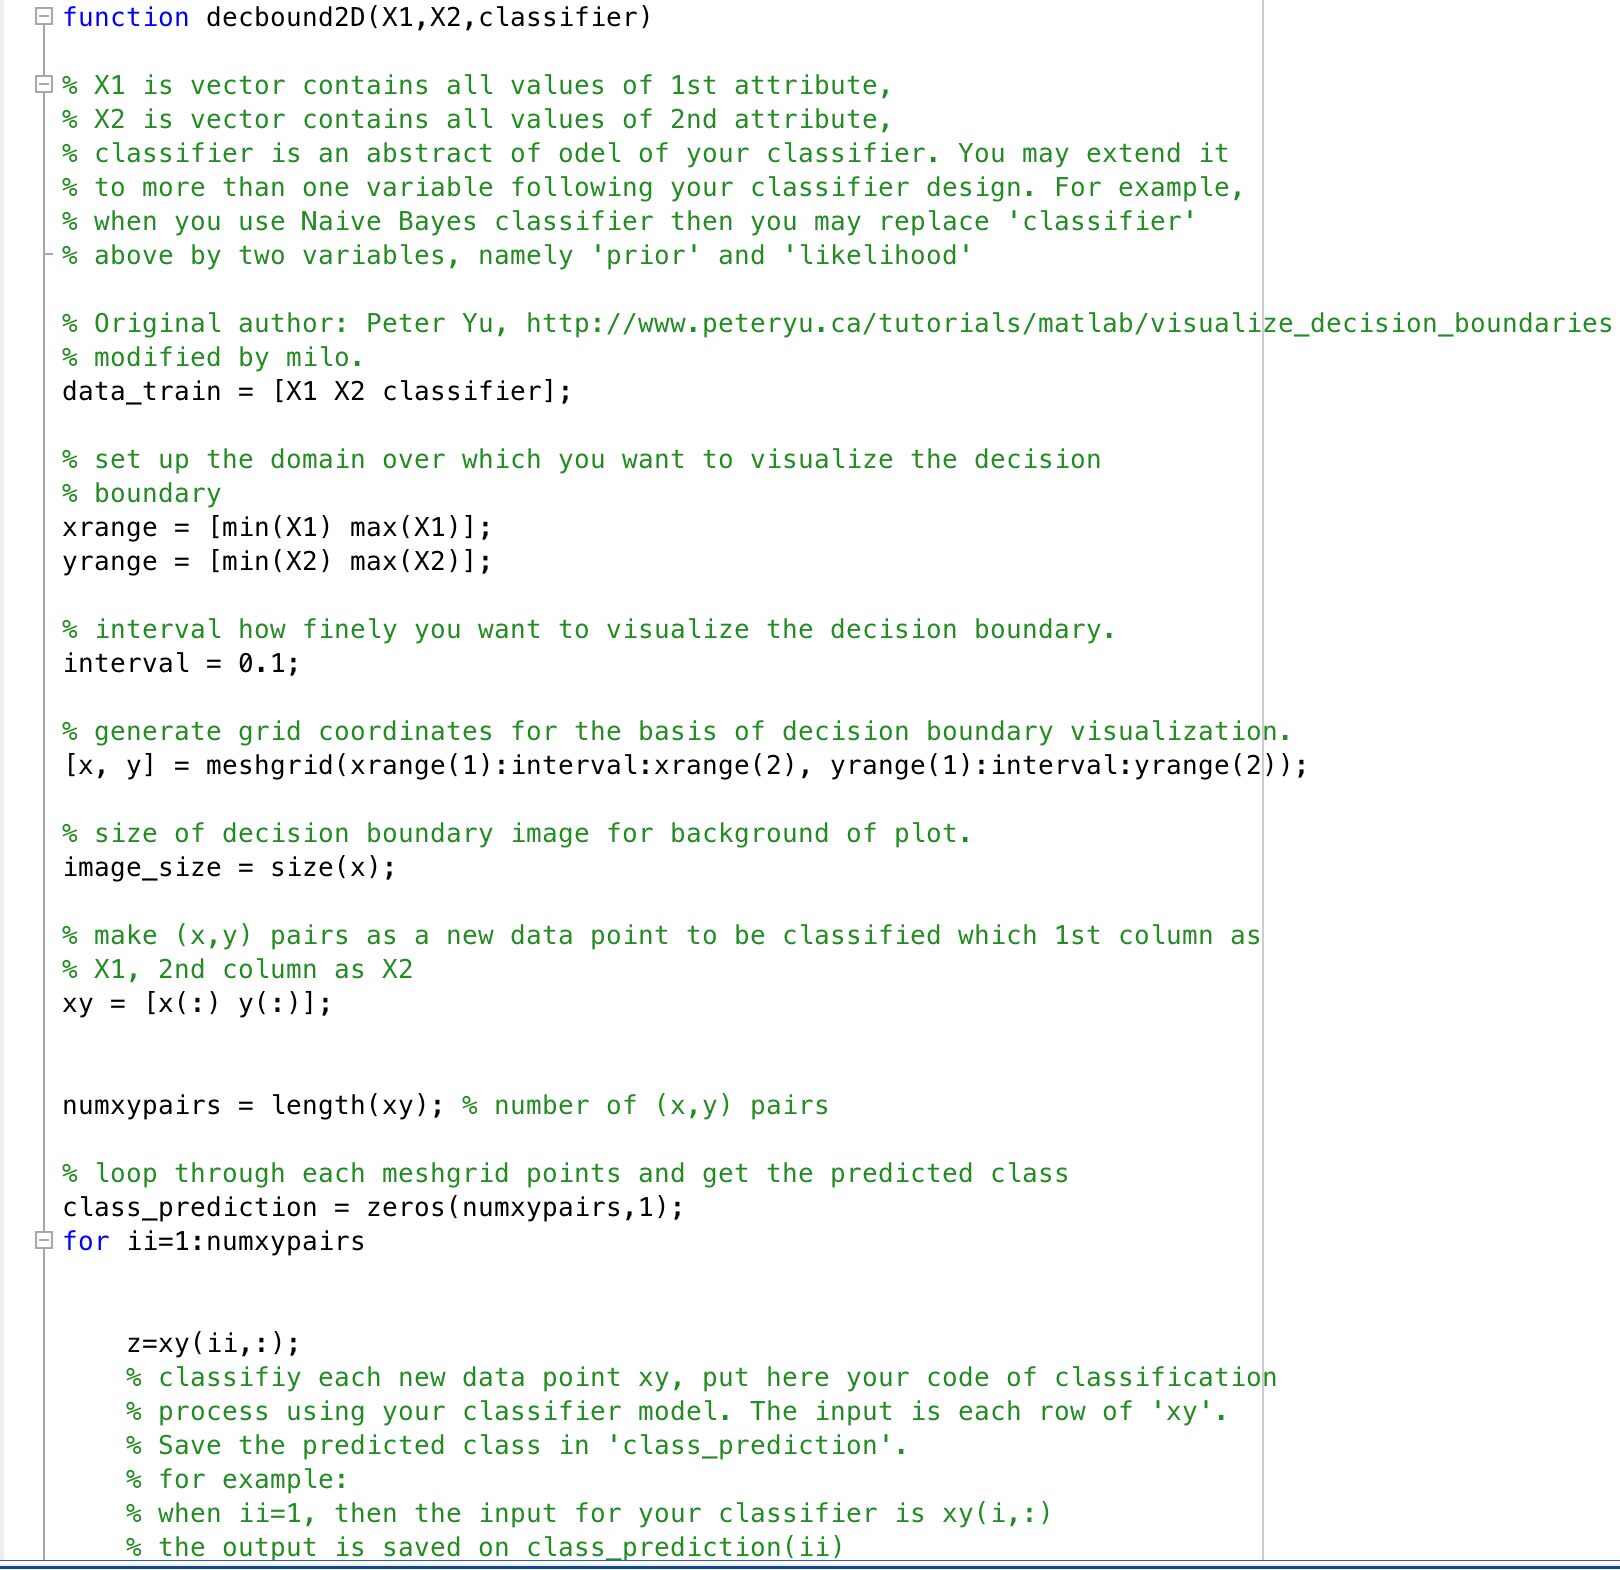
\includegraphics[width=10cm]{ass2clo3no19_6}
		\par 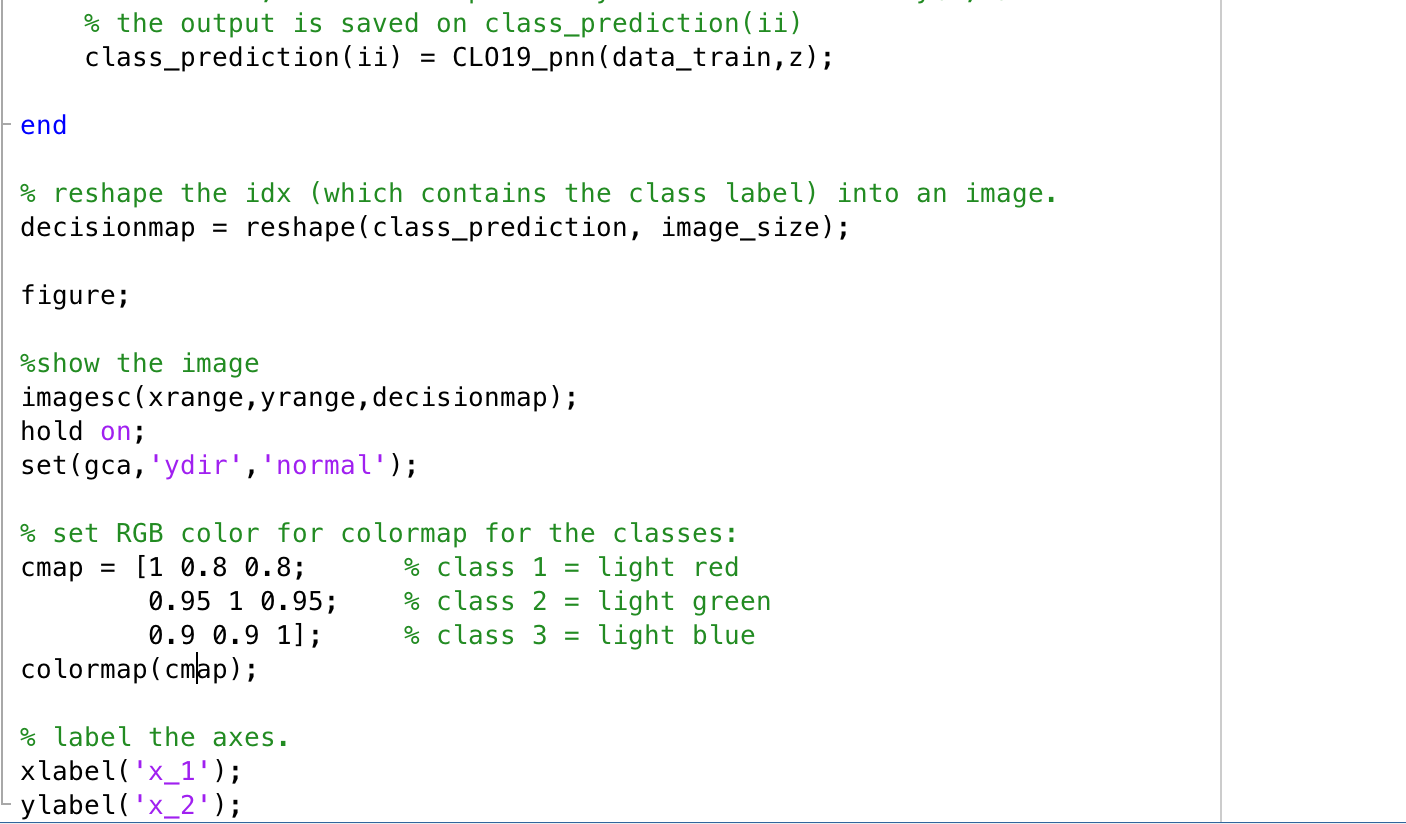
\includegraphics[width=10cm]{ass2clo3no19_7}  

		\par Ketika fungsi tersebut di-plot pada figur 19(a) ditambah dengan mencoba fungsi PNN dengan data\_test acak, maka didapatkan :
		\par 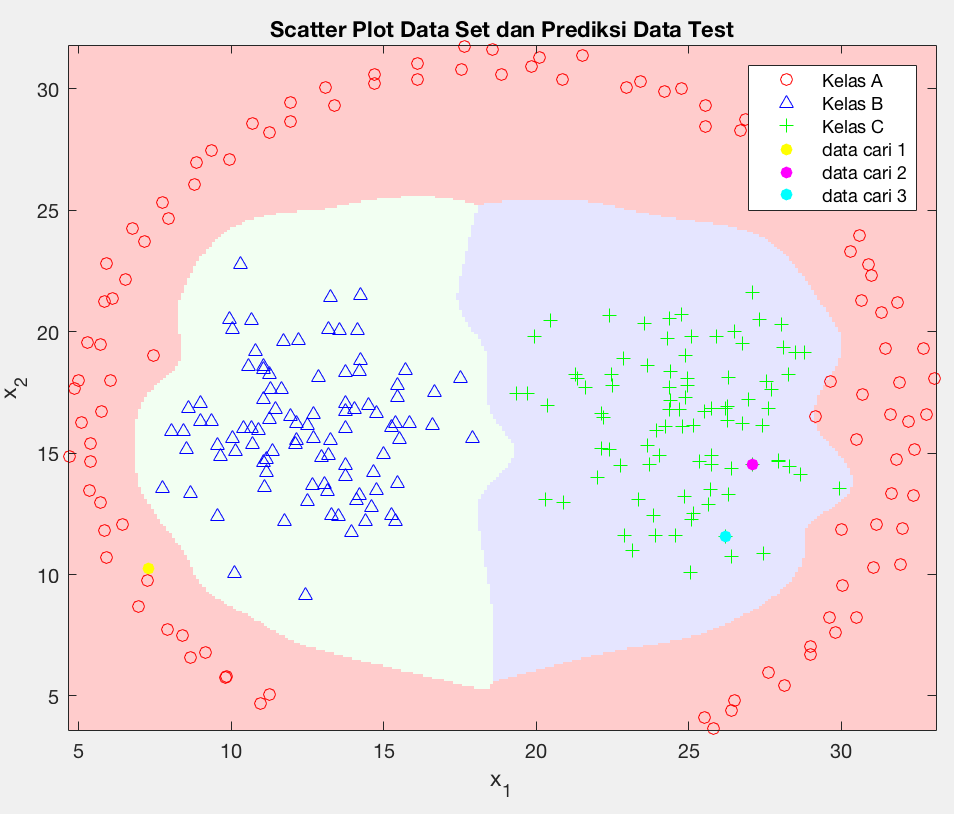
\includegraphics[width=10cm]{ass2clo3no19_8}
		\par 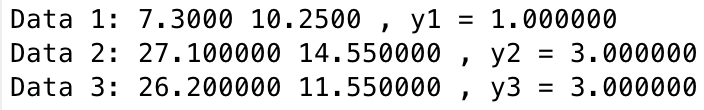
\includegraphics[width=10cm]{ass2clo3no19_9}  

		\item (5 points) How good is the classification result on test set? Give your opinion.
		\par Berdasarkan hasil beberapa kali \texit{testing}, \textit{classifier PNN} selalu berhasil mengklasifikasikan data dengan benar. Jadi menurut saya, \textit{classifier} dengan PNN sangat bagus.
 
	\end{enumerate}
	


\end{enumerate}

\par \textbf{Referensi}
\par [1] https://id.wikipedia.org/wiki/Regresi\_Linier
\par [2] Introduction to Data Mining - Panning Tan, M. Steinbach
\par [3] https://en.wikipedia.org/wiki/Nonlinear\_regression
\par [4] Regression book
\par [5] Regression slide
\par [6] http://www.nickgillian.com/wiki/pmwiki.php/GRT/MLP
\par [7] Machine Learning - Tom Mitchell
\par [8] https://medium.com/towards-data-science/activation-functions-and-its-types-which-is-better-a9a5310cc8f
\par [9] Slide ANN-MLP Machine Learning
\par [10] https://www.mathworks.com/help/optim/ug/quadprog.html#inputarg\_f
\par [11] http://www.robots.ox.ac.uk/~az/lectures/ml/ matlab2.pdf
\par [12] https://se.mathworks.com/matlabcentral/ answers/104248-implementation-support-vector-machine-nonlinear-case-with-quadprog- function-in-matlab


\end{document}

